\documentclass[tikz,border=5mm]{standalone}
\usepackage{pgfplots}
\usepackage{amsmath}
\pgfplotsset{compat=1.18}

\definecolor{silverblue}{RGB}{0, 0, 128}
\definecolor{goldpurple}{RGB}{128, 0, 128}
\definecolor{regiongreen}{RGB}{175, 238, 175}
\definecolor{optred}{RGB}{204, 24, 66}

\begin{document}
	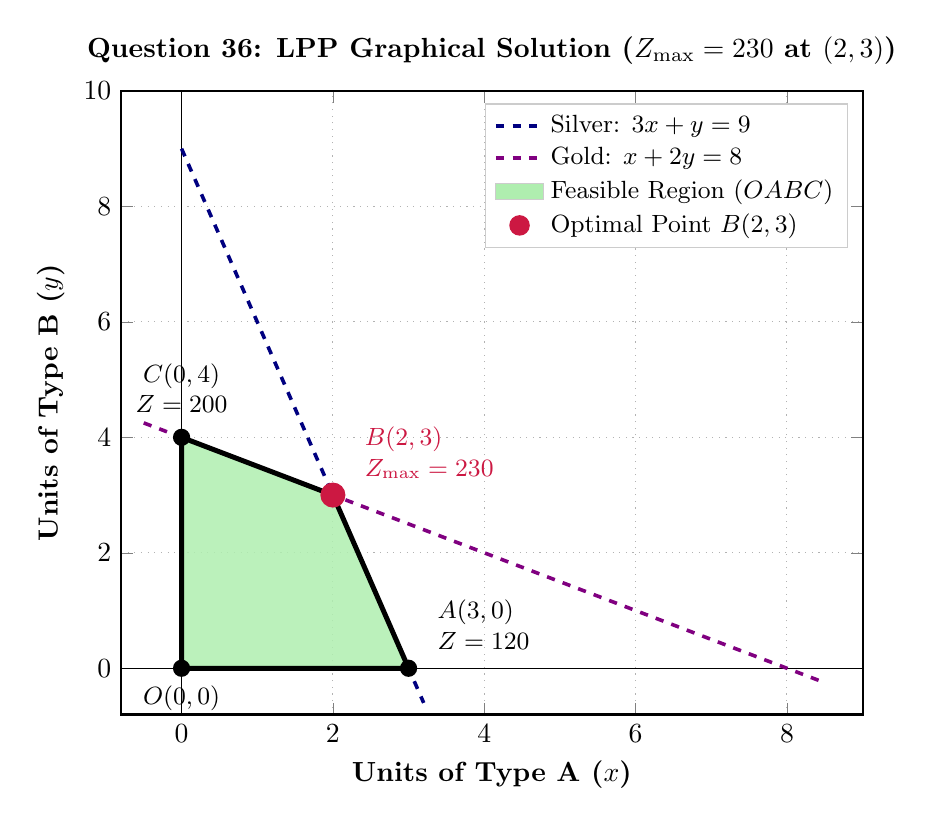
\begin{tikzpicture}
		\begin{axis}[
			width=11cm, height=9.5cm,
			title={\textbf{Question 36: LPP Graphical Solution ($Z_{\max} = 230$ at $(2, 3)$)}},
			xlabel={\textbf{Units of Type A ($x$)}},
			ylabel={\textbf{Units of Type B ($y$)}},
			xmin=-0.8, xmax=9.0,
			ymin=-0.8, ymax=10.0,
			xtick={0, 2, 4, 6, 8},
			ytick={0, 2, 4, 6, 8, 10},
			grid=both,
			grid style={dotted, gray!60},
			axis line style={black, thick},
			legend cell align={left},
			legend style={at={(0.98,0.98)}, anchor=north east, font=\small, draw=gray!40}
			]
			% Origin axis lines
			\draw[black, thin] (axis cs:0,-0.8) -- (axis cs:0,10);
			\draw[black, thin] (axis cs:-0.8,0) -- (axis cs:9,0);
			
			% Shaded Feasible Region (OABC)
			\fill[fill=regiongreen, opacity=0.85] (axis cs:0,0) -- (axis cs:3,0) -- (axis cs:2,3) -- (axis cs:0,4) -- cycle;
			
			% Constraint 1: 3x + y = 9  =>  y = 9 - 3x
			\addplot[silverblue, dashed, line width=1.3pt, domain=0:3.2] {9 - 3*x};
			\addlegendentry{Silver: $3x + y = 9$}
			
			% Constraint 2: x + 2y = 8  =>  y = 4 - 0.5x
			\addplot[goldpurple, dashed, line width=1.3pt, domain=-0.5:8.5] {4 - 0.5*x};
			\addlegendentry{Gold: $x + 2y = 8$}
			
			% Feasible region legend
			\addlegendimage{area legend, fill=regiongreen, draw=none}
			\addlegendentry{Feasible Region ($OABC$)}
			
			% Optimal Point legend
			\addlegendimage{only marks, mark=*, mark size=3.5pt, optred}
			\addlegendentry{Optimal Point $B(2, 3)$}
			
			% Heavy boundary for feasible region
			\draw[black, line width=1.8pt] (axis cs:0,0) -- (axis cs:3,0) -- (axis cs:2,3) -- (axis cs:0,4) -- cycle;
			
			% Corner points
			\node[circle, fill=black, inner sep=2.2pt] at (axis cs:0,0) {};
			\node[below=2pt, font=\small] at (axis cs:0,0) {
				\begin{tabular}{c}
					$O(0, 0)$ \\ $Z = 0$
				\end{tabular}
			};
			
			\node[circle, fill=black, inner sep=2.2pt] at (axis cs:3,0) {};
			\node[anchor=south west, font=\small, xshift=1pt] at (axis cs:3,0) {
				\begin{tabular}{l}
					$A(3, 0)$ \\ $Z = 120$
				\end{tabular}
			};
			
			\node[circle, fill=black, inner sep=2.2pt] at (axis cs:0,4) {};
			\node[above=2pt, font=\small] at (axis cs:0,4) {
				\begin{tabular}{c}
					$C(0, 4)$ \\ $Z = 200$
				\end{tabular}
			};
			
			% Optimal Point B(2, 3)
			\node[circle, fill=optred, inner sep=3.2pt] at (axis cs:2,3) {};
			\node[anchor=south west, font=\small, text=optred, xshift=2pt] at (axis cs:2,3) {
				\begin{tabular}{l}
					\textbf{$B(2, 3)$} \\
					\textbf{$Z_{\max} = 230$}
				\end{tabular}
			};
		\end{axis}
	\end{tikzpicture}
\end{document}